\chapter{Inleiding}
\label{inleiding}
%%%%%%%%%%%%%%%%%%%%%%%%%%%%%%%%%%%%%%%%%%%%%%%%%%%%%%%%%%%%%%%%%%%%%%%%

\begin{center}
    \begin{minipage}{0.5\textwidth}
        \begin{small}
            Waar de reden tot creatie van dit verslag worden blootgelegd, de
            opdracht en het probleem worden beschreven en achtergrondinformatie
            word gegeven.
        \end{small}
    \end{minipage}
    \vspace{0.5cm}
\end{center}

\noindent EV Europe is een bedrijf dat werkt met klanten die gebruik willen
maken van de nieuwste technieken op het gebied van elektrische auto's. Zo word
er vaak door de klanten gevraagd of moderne snufjes kunnen worden ingebouwd in
hun auto. Recent was dat de vraag om langs de snelweg aan een snel laad paal te
kunnen laden. Deze palen (of \ac{evse}) maken in europa gebruik van het \ac{ccs}
protocol \cite{Directive_2014/94/EU}. Dus EV Europe is gaan onderzoeken of het
gebruik van deze \ac{ccs} snel laad palen een optie is voor de klanten en wat er
voor nodig is om dit te bereiken.

%%%%%%%%%%%%%%%%%%%%%%%%%%%%%%%%%%%%%%%%%%%%%%%%%%%%%%%%%%%%%%%%%%%%%%%%
\section{Achtergrond elektrische auto's}
%%%%%%%%%%%%%%%%%%%%%%%%%%%%%%%%%%%%%%%%%%%%%%%%%%%%%%%%%%%%%%%%%%%%%%%%

Er zijn grofweg twee soorten elektrische auto's (\ac{ev}), plug-in elektrische
auto's en hybride auto's. Plug-in elektrische auto's zijn auto's die alleen
elektrisch rijden, en hybride auto's zijn auto's die zowel elektrisch en op
verbrandingsmotor rijden (er zijn nog meer onderscheidingen zoals onder anderen
plug-in hybride en waterstofauto's die niet van toepassing zijn op dit
verslag).

EV Europe is vooral geïnterneerd in de eerste soort, de plug-in elektrische
auto's. De plug-in elektrische auto's zijn auto's met een volledig elektrische
aandrijflijn, en die dus ook elektrisch moeten worden opgeladen. De
aandrijflijn van deze auto's bestaat uit een accupakket, een motorcontroller,
en een elektromotor. De overigen mechanische componenten van de aandrijflijn
zijn vrijwel gelijk aan die van een interne verbrandingsmotor auto.

In de laatste jaren is de hoeveelheid elektrische auto's op de markt hard aan
het groeien. Bovendien de infrastructuur, zoals (snel)laaders. 

%%%%%%%%%%%%%%%%%%%%%%%%%%%%%%%%%%%%%%%%%%%%%%%%%%%%%%%%%%%%%%%%%%%%%%%%
\subsection{Laadden van elektrische auto's}
%%%%%%%%%%%%%%%%%%%%%%%%%%%%%%%%%%%%%%%%%%%%%%%%%%%%%%%%%%%%%%%%%%%%%%%%

Het laden van EV's gaat wereldwijd door middel van verschillende standaarden,
maar in europa hebben het \ac{ccs} systeem geadopteerd. Ondanks de andere
standaarden die nog steeds hier en daar ondersteund worden, focussen we ons in
dit verslag volledig op het \ac{ccs} systeem.

%%%%%%%%%%%%%%%%%%%%%%%%%%%%%%%%%%%%%%%%%%%%%%%%%%%%%%%%%%%%%%%%%%%%%%%%
\subsection{\ac{ccs} laden}
%%%%%%%%%%%%%%%%%%%%%%%%%%%%%%%%%%%%%%%%%%%%%%%%%%%%%%%%%%%%%%%%%%%%%%%%

\ac{ccs} laden kan met AC en met DC, afhankelijk van de \ac{evse} en de opties
op de auto kan er AC of DC worden geladen. AC laden staat wel beschreven in de
\ac{ccs} standaard, echter word het AC laden met de type 2 stekker vaak niet
\ac{ccs} genoemd maar gewoon AC. Er zijn dus twee soorten \ac{ccs} laden: AC en
DC.

Er zijn ook twee soorten stekkers (de kant van de \ac{evse} ook wel outlet
genoemd) en twee soorten inlet's (de kant van de \ac{ev}). De Combo 2 stekker
(zie figuur \ref{fig:CCS_combo2_outlet}) ondersteund alleen DC laden, maar de
Combo 2 inlet (zie figuur \ref{fig:CCS_combo2_inlet}) ondersteund over het
algemeen zowel AC als DC laden. Verder zijn de type 2 stekker (zie figuur
\ref{fig:AC_type2_inlet_outlet}) en inlet (zie figuur
\ref{fig:AC_type2_inlet_outlet}) alleen voor AC laden

\begin{figure}[h]
    \centering
    \begin{minipage}{0.45\textwidth}
        \centerline{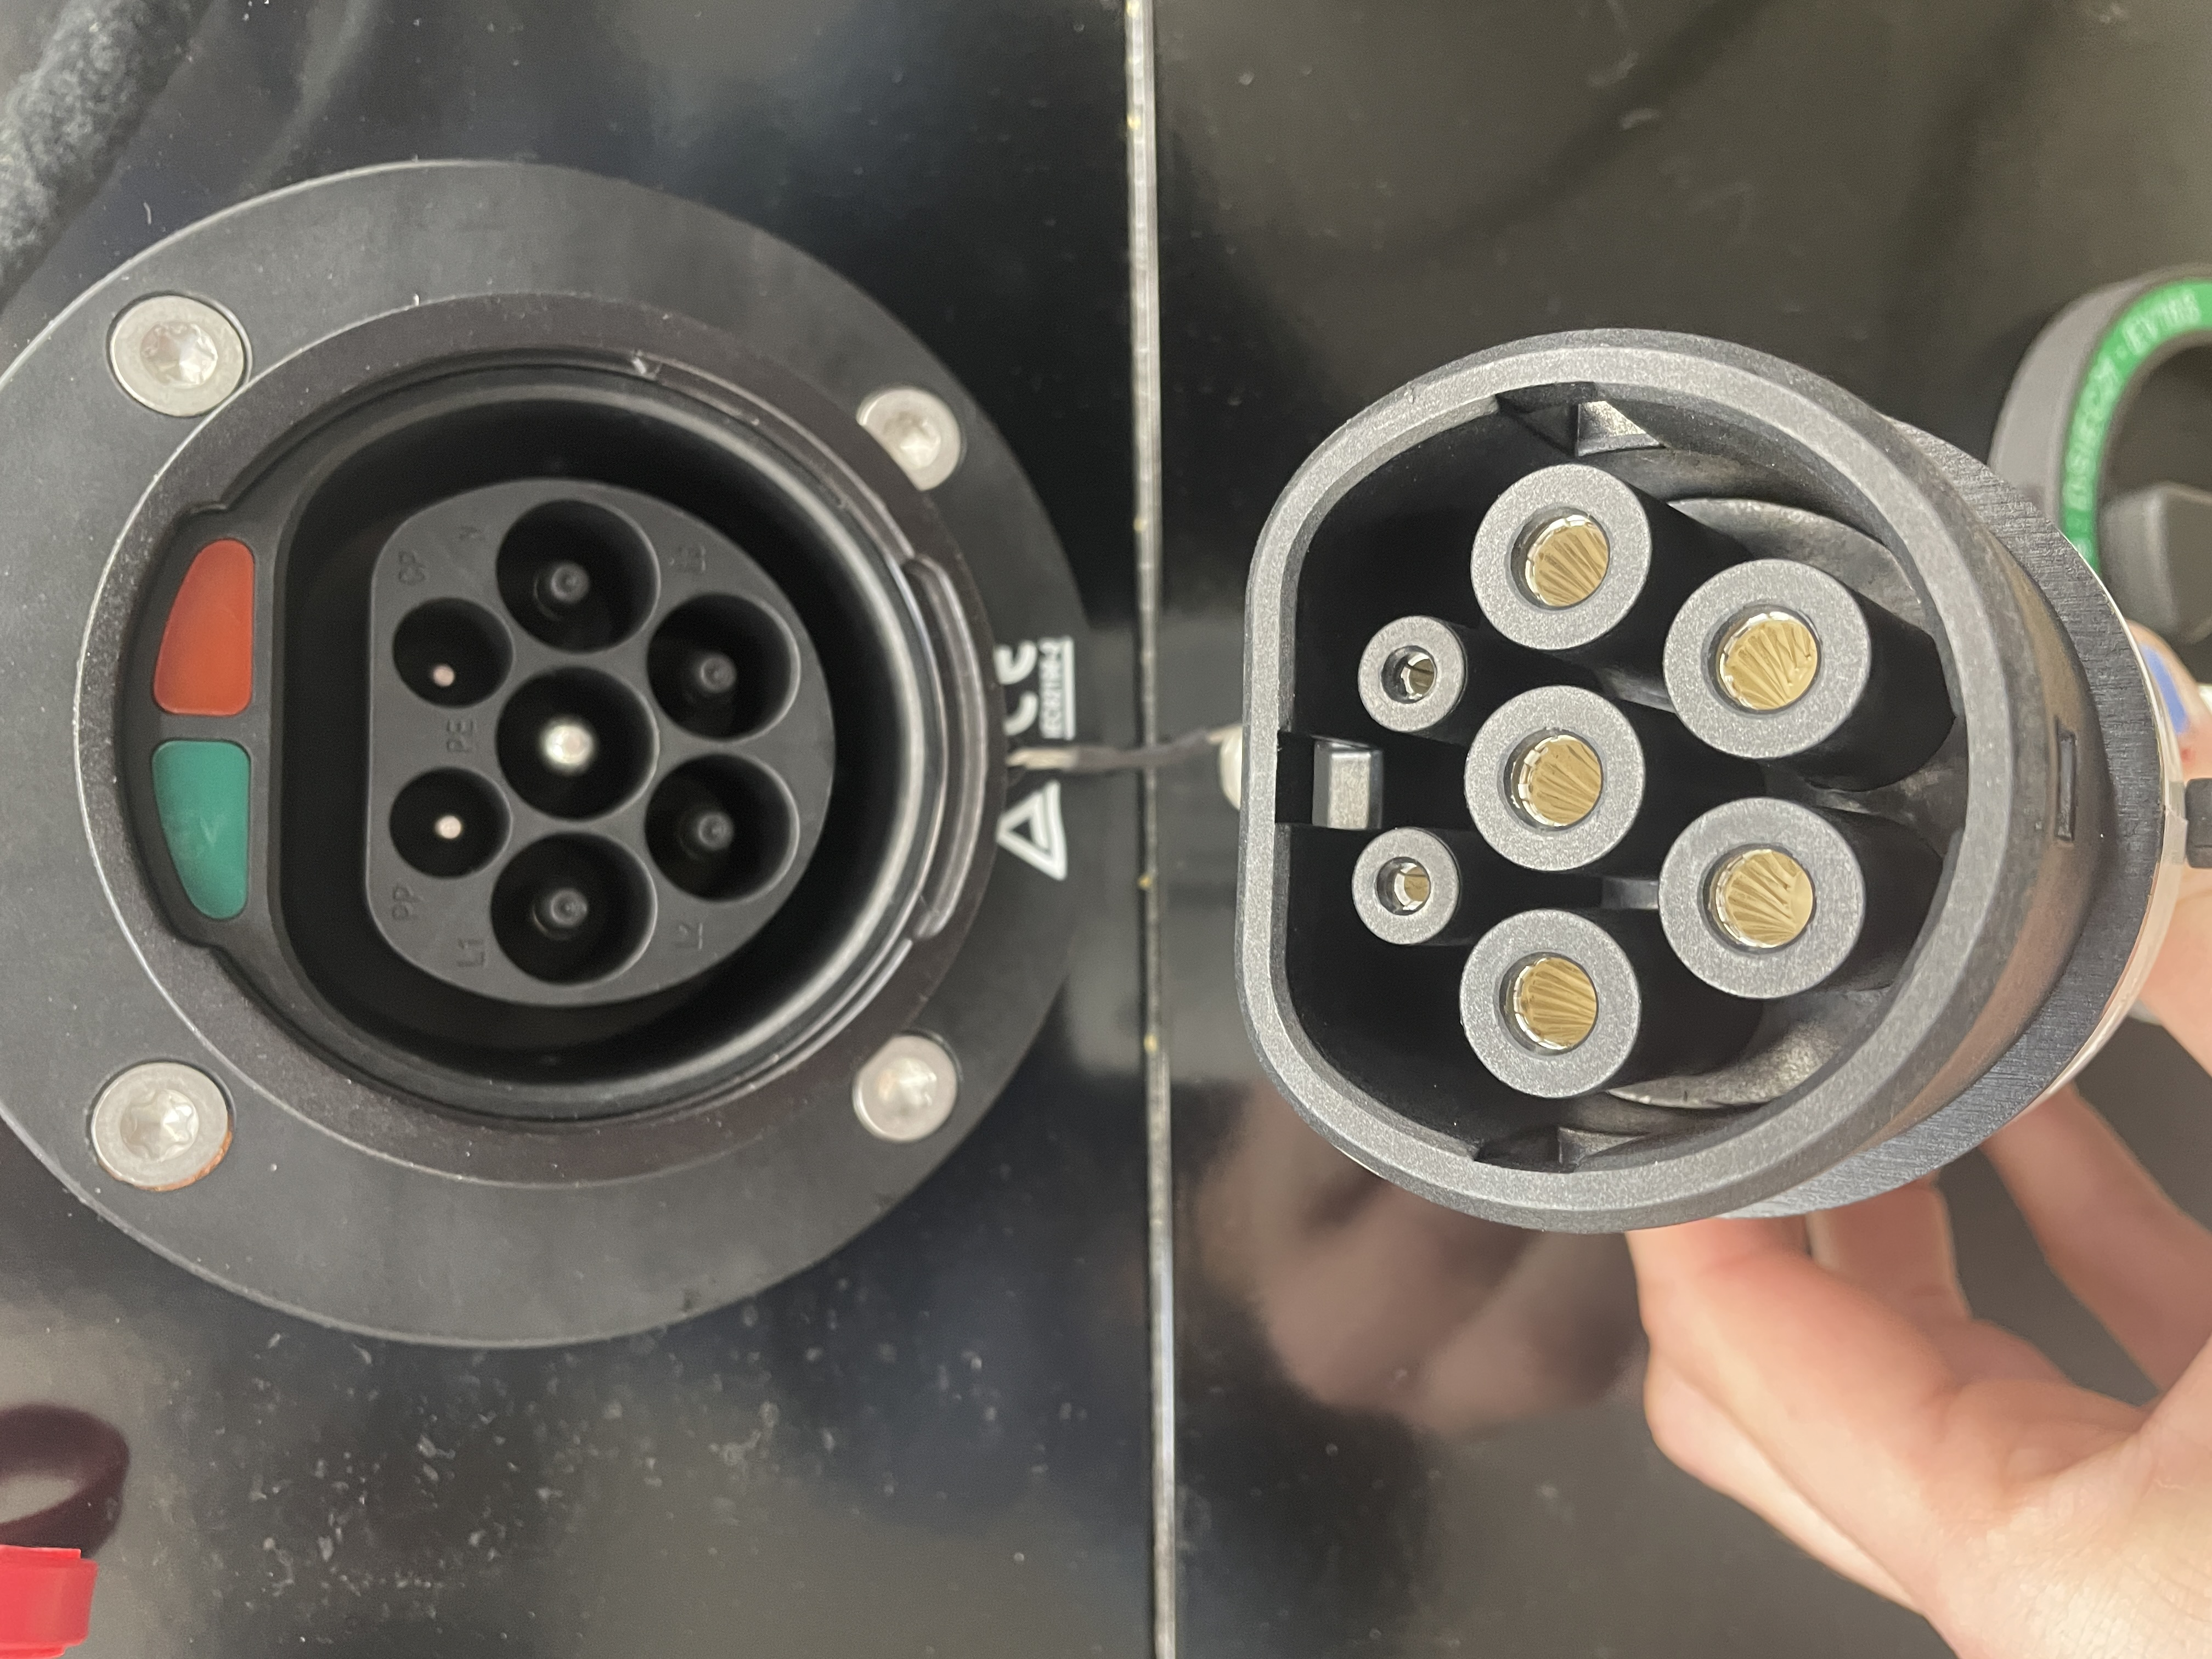
\includegraphics[width=0.9\textwidth,angle=-90]{AC_type2_inlet_outlet}}
        \caption{AC Type 2 inlet (boven) en outlet (onder)}
        \label{fig:AC_type2_inlet_outlet}
    \end{minipage}\hfill
    \begin{minipage}{0.45\textwidth}
        \centerline{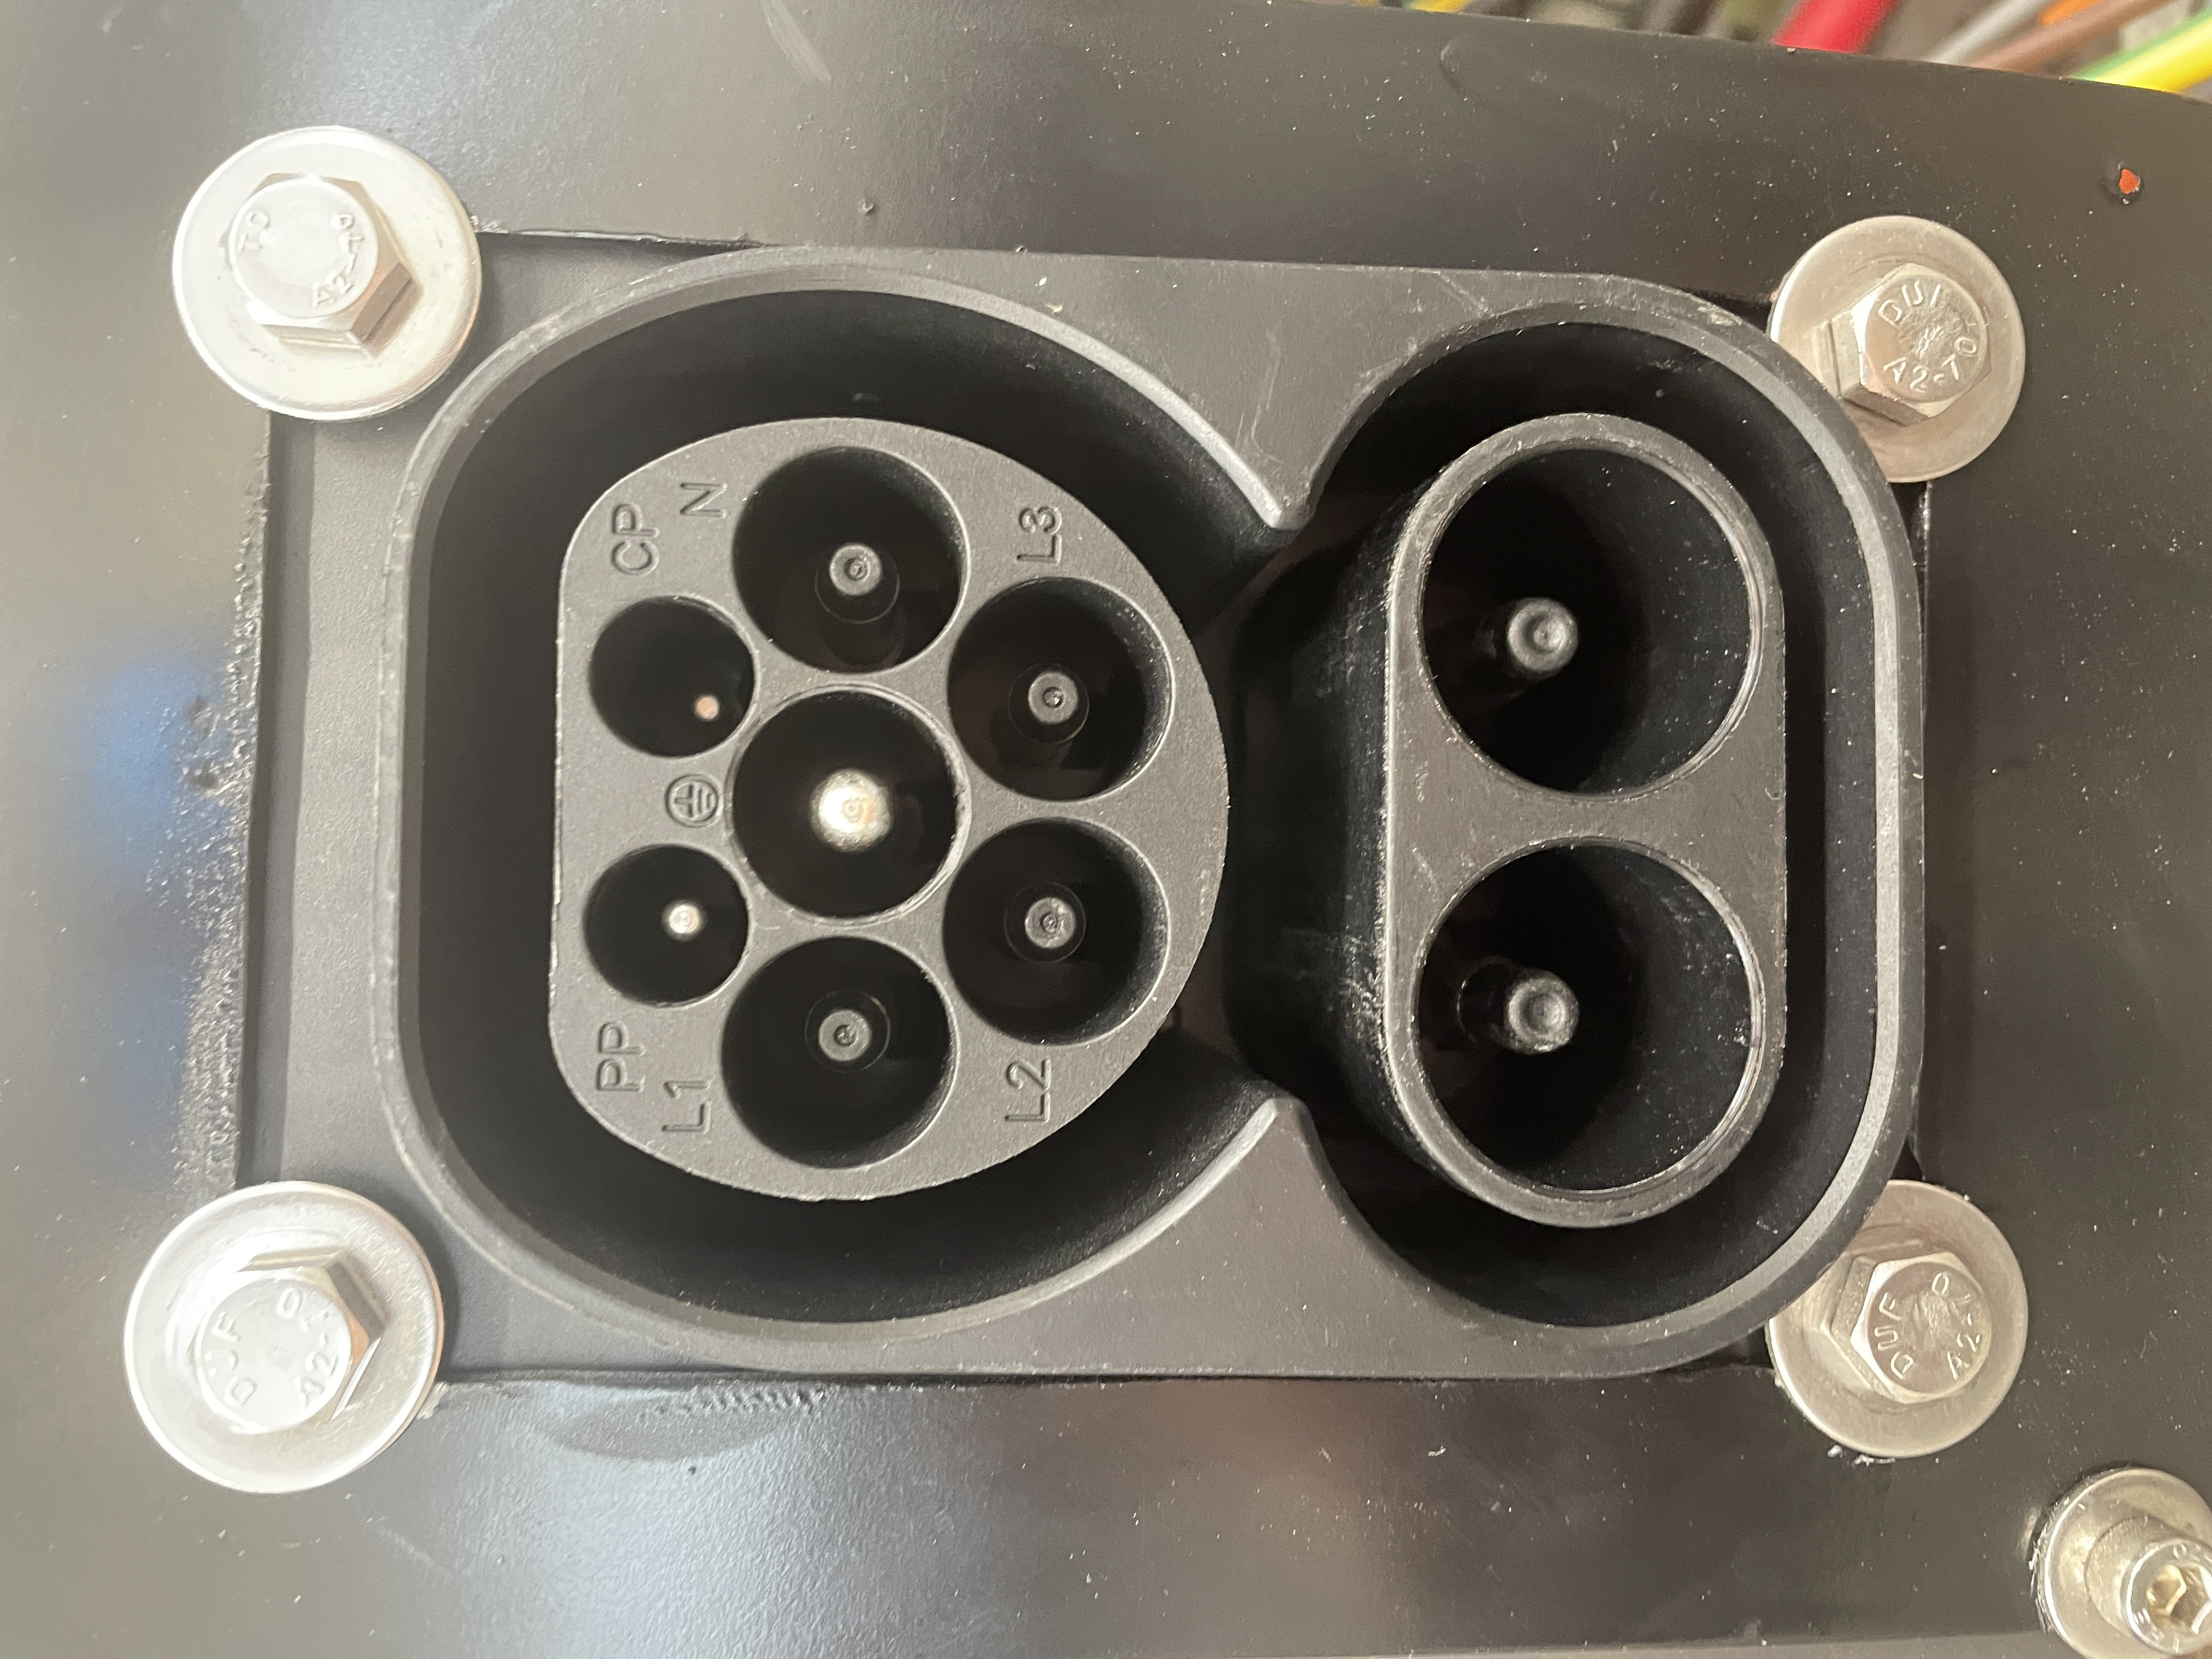
\includegraphics[width=0.9\textwidth,angle=-90]{CCS_combo2_inlet}}
        \caption{CCS Combo 2 inlet}
        \label{fig:CCS_combo2_inlet}
        \hfill
        \centerline{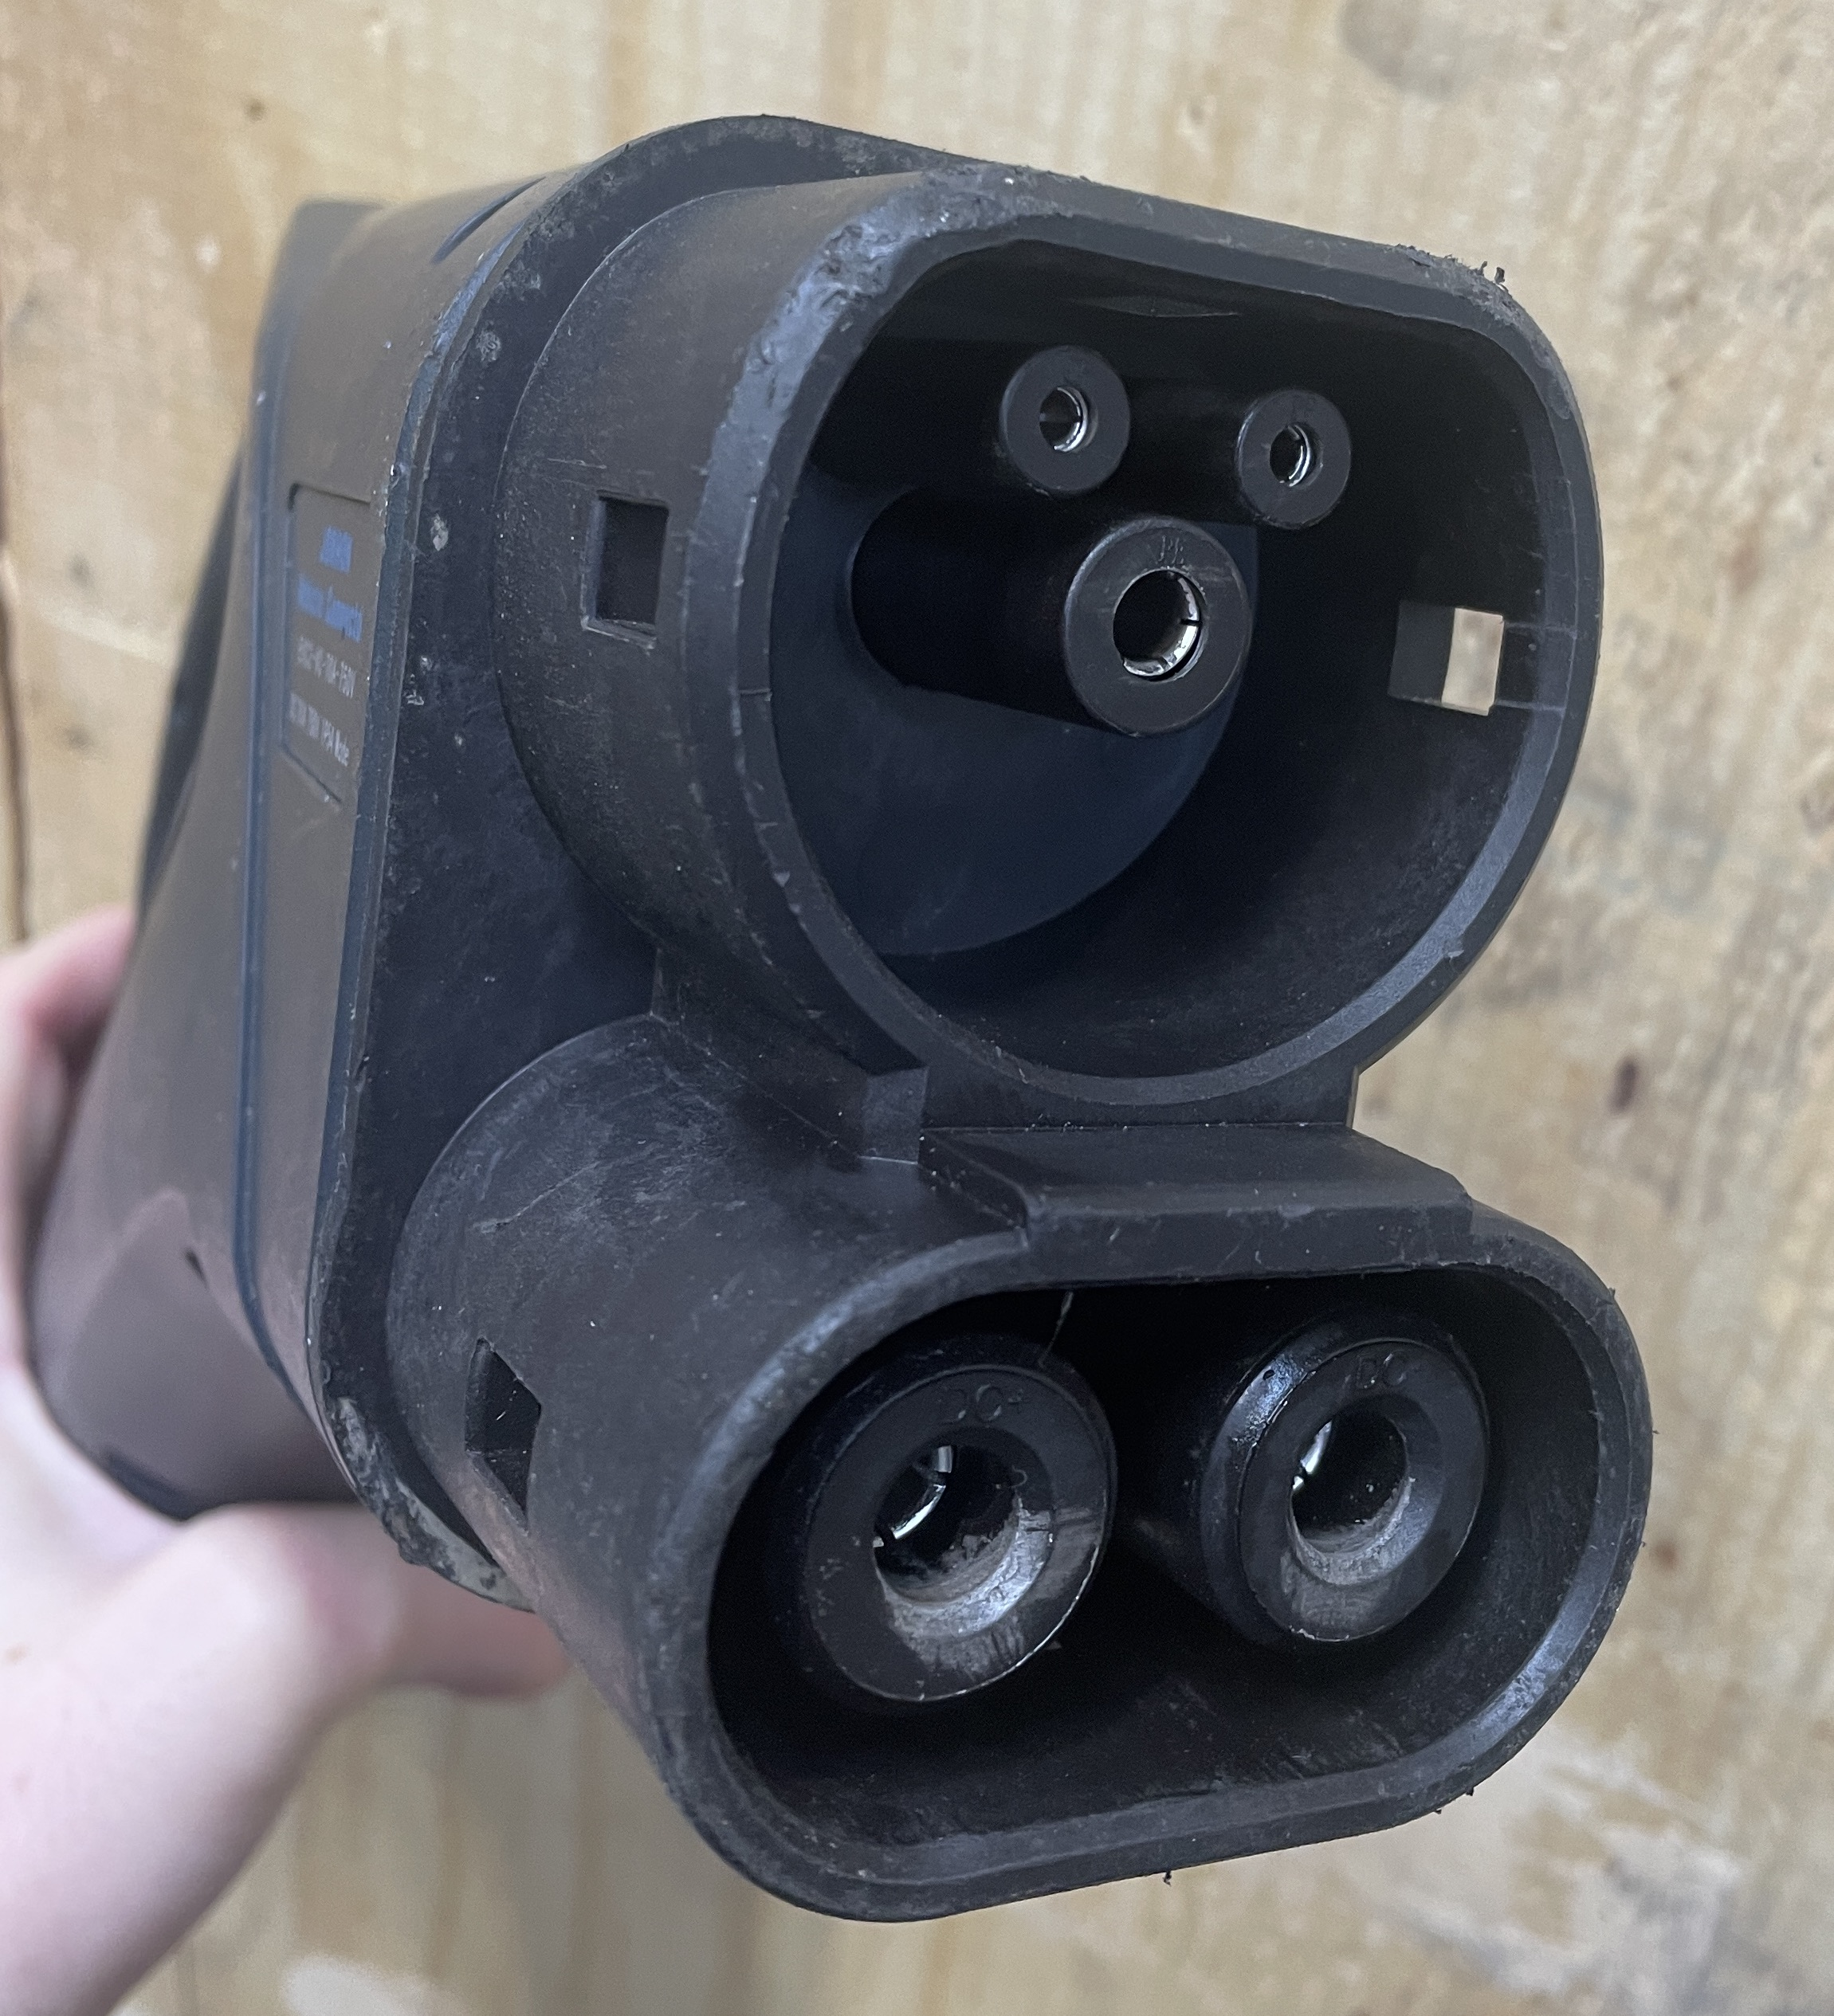
\includegraphics[width=0.9\textwidth]{CCS_combo2_outlet}}
        \caption{CCS Combo 2 outlet (stekker)}
        \label{fig:CCS_combo2_outlet}
    \end{minipage}
\end{figure}

%%%%%%%%%%%%%%%%%%%%%%%%%%%%%%%%%%%%%%%%%%%%%%%%%%%%%%%%%%%%%%%%%%%%%%%%
\subsubsection{AC laden}
%%%%%%%%%%%%%%%%%%%%%%%%%%%%%%%%%%%%%%%%%%%%%%%%%%%%%%%%%%%%%%%%%%%%%%%%

\ac{ac} laden kan ook nog op verschillende manieren en snelheden, het grootste
verschil is een fase en drie fasen, waarbij drie fasen in principe drie keer zo
snel kan laden als een fase. Deze laadmethode gebruikt een interne lader in de
auto (\ac{ev}). En de communicatie tussen de auto en de \ac{evse} is heel
simpel met een \ac{pwm} signaal. Het \ac{pwm} signaal word gebruikt om de
maximale stroom die de \ac{evse} kan leveren te communiceren aan de \ac{ev}. De
\ac{ev} geeft dan een signaal dat de \ac{ev} klaar is om te laden en de
\ac{evse} zet dan netspanning (een of drie fasen) op de te poolen van de type 2
stekker (outlet).

%%%%%%%%%%%%%%%%%%%%%%%%%%%%%%%%%%%%%%%%%%%%%%%%%%%%%%%%%%%%%%%%%%%%%%%%
\subsubsection{DC laden}
%%%%%%%%%%%%%%%%%%%%%%%%%%%%%%%%%%%%%%%%%%%%%%%%%%%%%%%%%%%%%%%%%%%%%%%%

\ac{dc} laden word dus CCS laden genoemd. De \ac{evse} gebruikt de Combo 2
outlet (stekker) en de \ac{ev} gebruikt de Combo 2 inlet. De \ac{evse} is bij
DC laden de lader, en wordt door middel van contactoren in de \ac{ev} direct
aan de accupolen aangesloten. Hiermee kan met veel hogere stroom worde geladen
en daarom word \ac{dc} laden ook wel snelladen genoemd.